\chapter{Related Work}
\label{ch:relWork}

This chapter will outline some of the past approaches to solve the task of Sentiment Analysis and Aspect Based Sentiment Analysis, as well as more recent approaches to give a general overview of the field. While the first section will deal with the traditional task of sentiment extraction, section~\ref{sec:02_absa} will discuss linking sentiment to specific aspects.

\section{Sentiment Analysis}

Traditionally, sentiment analysis has been approached by carfully engineering features which were handtuned to a specific work task. Most approaches used either rule based systems \cite{Popescu2005} or lexicons to find the sentiment polarity of a document. Huettner and Subasic use a word lexicon for semantic categiues and a word affection lexicon with 4000 words. Each word in the lexicon is then assigned one category \cite{Huettner2000}. 

Das and Chen use a similar approach where they manually compile a word lexicon. They use those words in combination with scoring functions to classify user generated posts on stock-market message boards as \textit{bullish} {(positive for the stockmarket)} or \textit{bearish} {(negative for the stock market)} \cite{Das2007}.

Hu and Liu improve upon the tedious task of building a lexicon by using only a small ammount of seed adjectives which is grown by the use of wordNet \cite{Hu2004}.
\medskip

Lexicon based approaches are often manually build for a specific task like movie reviews \cite{Tong2001, Thet2010} and therefore, generally domain dependet. For instance, sentiment in movie reviews is expressed very differently compared to a product or restaurant review. On the other hand, general sentiment lexicons like SentiWordNet \cite{Baccianella2010} are mostly to general to successfully capture domain specific sentiment.
\medskip

Tourney uses an unsupervised system which classifies the sentiment of reviews as thumbs up or thumbs down. This is done by computing the closest association of adjectives and adverbs in a sentence. They then comopare the number of positive associations {(associations to words like \textit{good} or \textit{romantic})} in a sentnece to the amount of negative associations {(words like \textit{horrific})} \cite{Turney2007}.
\medskip

In 2012 Pang et. al. compare traditional machine learning techniques {(Naive Bayes classifier, maximum entropy classification and \glspl{svm})} with human feature engineered baselines on movie reviews \cite{Pang2012}. They still use word lists to classify the polarity of a sentence but they conclude that a sentiment lexicon generated by a machine learning algorithm always outperforms manually created lexicons.
\medskip


Usually, lexicon approaches used to work in combination with scoring functions where the most trivial ones would just sum up the negative and positive words in a document. The algorithm would classify a document as positive if the sum of positive words is positive. However, there are limitations to this technique since sentences are often tree structured and may contain negated sub-trees. Just counting the positive and negative words in the sentence "\textit{This film doesn't care about cleverness, wit or any other kind of intelligent humor}" would yield in a highly positive sentiment since it does not take the negation into account. Socher et al. introduce a "recursive neural tensor network" \cite{Socher2013}. "Recursive neural networks" or "tree-structured neural networks" use the output of a forward pass as the input and some additional information as a new forward pass. By treating each word as a node in a tree they are able to input a subtree into the network, get the output and then use this output and the words on the next layer as the new input until the root node is reached. With this technique they are able to capture contrastive sentences where the first half contains negative sentiment and the second half positive sentiment in addition to negated sentiment. 
\medskip

\section{Aspect Based Sentiment Analysis}
\label{sec:02_absa}

\acrfull{absa} takes Sentiment Analysis one step further. Instead of just predicting sentiment for a sentence of document, \gls{absa} predicts sentiment for a specific aspect. This solves a major dilemma for normal sentiment analysis when a sentence or document contains multiple contradictive sentiments. For instance, the sentence "\textit{The food tasted great but the price was too high}" contains two conflicting sentiment instances {(Positive: great food - Negative: High Price)}. A classifier just modelling sentiment anaylsis would have to label this sentence as beeing neutral whereas an \gls{absa} system could classify the aspect \textit{food} as positive and \textit{price} as negative. In addition \gls{absa} is also much more useful for consumers and companies alike as discussed in the previous section.
\medskip

\subsection{Datasets}

There are several datasets which provide tasks that include \gls{absa}. Most widely used are the SemEval datasets. Task 4 of SemEval-2014 contains 7686 annotated sentences about restaurants and laptops \cite{Pontiki2014}. 

Task 12 of SemEval-2015 expands the dataset of the previous year with the category hotels \cite{Pontiki2015a}. 

Lastly, Task 5 of SemEval-2016 adds additional subtasks for \gls{absa} and text-level aspect-sentiment extraction as well as two new domains in different languages \cite{Pontiki2015a}. In addition they also provide a task where classifiers have to perform out-of-domain \gls{absa}. Unfortunatelly, there were no submissions for this subtask. This is one of the most challenging tasks. Even modern deep learning architectures still struggle to successfully classify outside of the domain they were trained on.
\medskip

Since annotating \gls{absa} datasets is very expensive in term of annotation costs, even the biggest SemEval datasets only contain less than 10,000 sentences over all splits. In contrast, GermEval-2017 is a shared task dataset which contains more than 25,000 comments \cite{Wojatzki2017}.  

\subsection{Deep Learning on \gls{absa}}

One crucial element for deep neural network training on natural language is the ability to transform a sequence of words from sparse high dimesional vectors to dense sentence embeddings. The majority of recent publications on \gls{absa} use sentence embeddings as their first input layer \cite{Ruder2016, Tang2016, Lee2017, Schmitt2018, Ma2018, Xue2018} in combination with \gls{lstm} architectures \cite{Ruder2016, Tang2016, Ma2018}.
\medskip

In most approaches reasearches use a pipeline procedure to perform \gls{absa}. During the first step, the models usually try to predict the aspects of the document. Then, in the second step of the pipeline the polarity is classified \cite{Lakkaraju2014}. The winner of GermEval-2017 task-C use a pipeline approach \cite{Lee2017} as well as three of the top performing approaches of SemEval-2016 \cite{Brun2016, Kumar2016, Xenos2016}.
\medskip

Lakkaraju, Socher and Manning investigate the influence of pipeline approaches against joint aspect and sentiment classification \cite{Lakkaraju2014}. They argue that combining aspect and sentiment detection gives a model the possibility to capture dependencies between aspect and sentiment more efficiently. They demonstrate that their joint aspect sentiment model using parse trees and \glspl{rnn} outperforms their pipeline baseline. To explain this they give several examples from the beer \cite{McAuley2012, McAuley2013b} and camara-reviews dataset they use. 

\begin{itemize}
	\item "{[...]} delicious beer that’s highly drinkable" - {(Palate : Positive)}
	\item "high carbonation level, kinda thin" - {(Palate : Negative)}
	\item "Display quality ofthe camera is high" - {(Display : Positive)}
	\item "This camera is highly expensive" - {(Price : Negative)}
\end{itemize}

Each of the four sentences contains the word "\textit{high}" but in each sentence it appears in a different form and may lead to both positive and negative sentiment depending on the aspect. Lakkaraju et. al. state that due to the aspect-sentiment linkage the single sentiment approach was not able to correctly classify those sentences whereas their joint aspect sentiment model predicted correctly.
\medskip

Ruder et. al. use a hierarchical, bidirectional \gls{lstm} for \gls{absa} \cite{Ruder2016}. Although they also assume a pipeline approach where aspects have to be fed in one after another they propose a interesting architecture. Usually, sentiment analyisis in combination with aspect detection is either done by having multiple heads for each aspect \cite{Schmitt2018} or by using a big softmax layer with every possible combination of aspect and sentiment which runs into issues when classifying multiple aspects at the same time \cite{Lakkaraju2014}. Ruder et. al. propose a third alternative where the aspect itself is fed into the network as an embedding alongside the actual text. After feeding the sentence embeddings through one bidirectional \gls{lstm} the text features and the aspect embedding are combined again. Together they are passed to the last bidirectional \gls{lstm} layer and classified in a last output layer. They report competitive results against two non-hierarchical baselines and achieve state of the art for multi-domain datasets.
\medskip
\begin{figure}[htp]
	\centering
	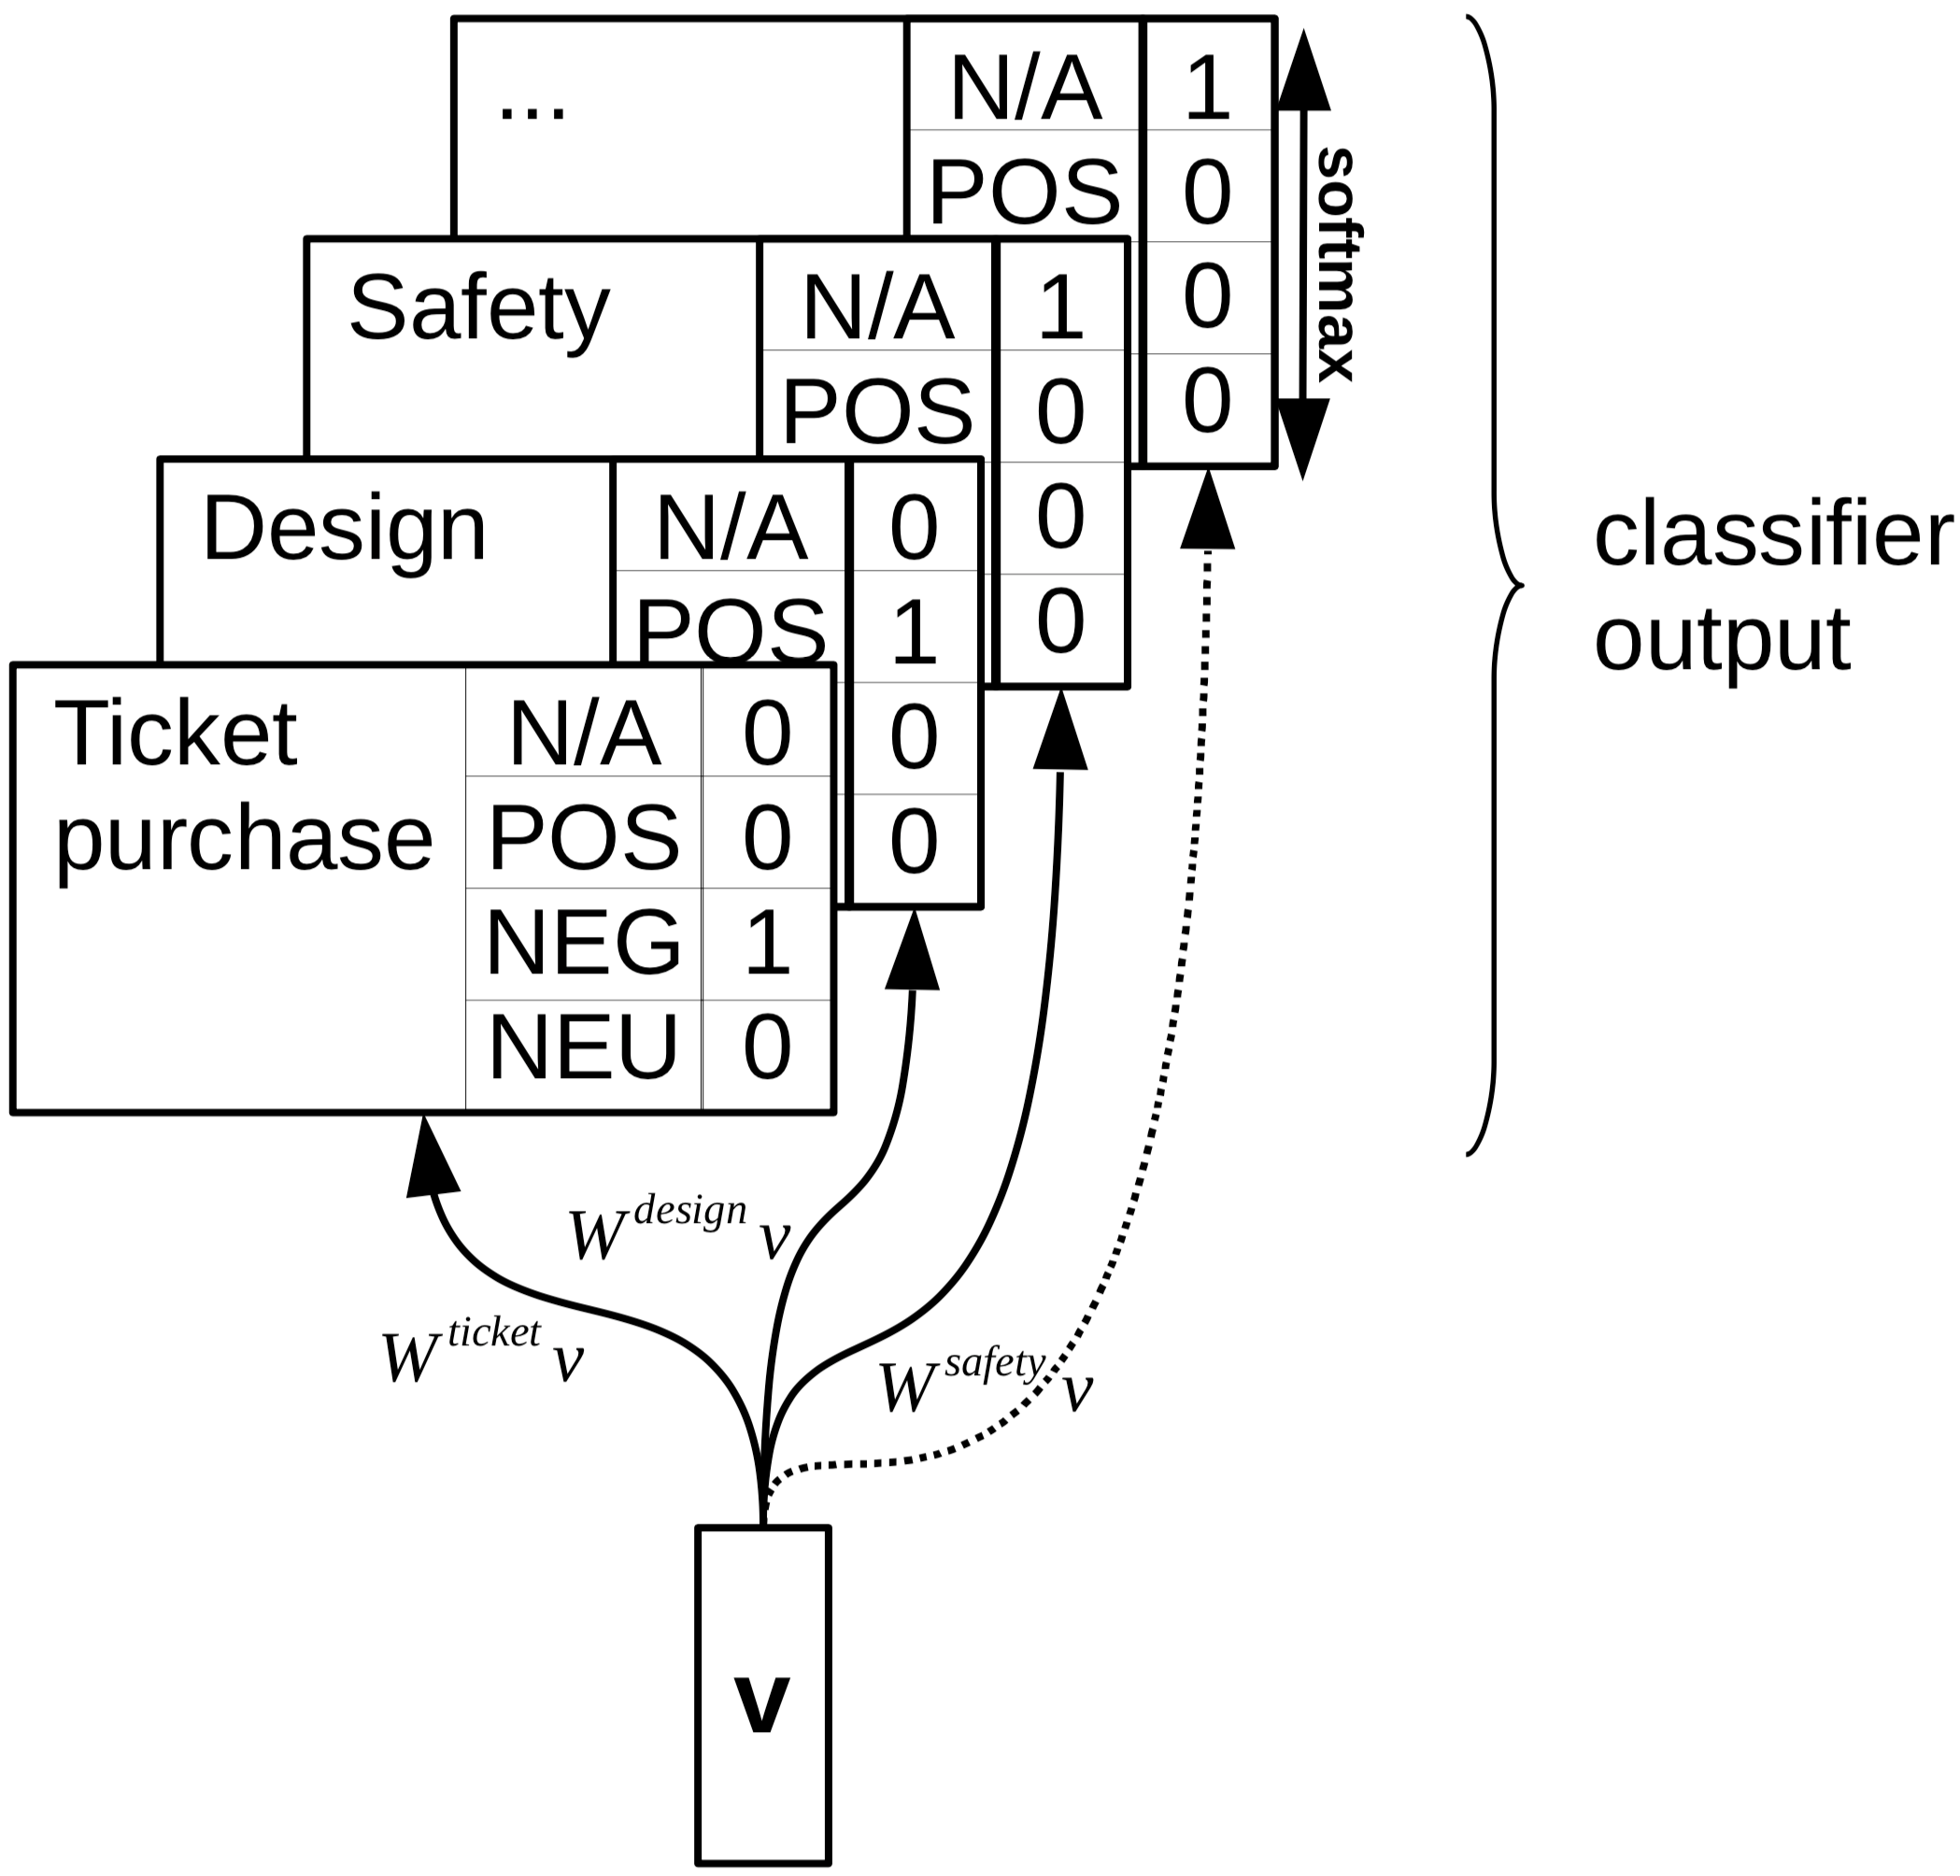
\includegraphics[width=0.5\textwidth]{figures/02_relatedWork/02_jabsa}
	\caption{Aspect Heads proposed by Schmitt et al. Source: Schmitt et. al. \cite{Schmitt2018}}
	\label{fig:02_j-absa}
\end{figure}

In 2018 Schmitt et. al. propose a novel approach to classify aspect and sentiment jointly \cite{Schmitt2018}. Similar to Lakkaraju they also compare joint-approaches and pipeline approaches. In both instances the joint approaches significantly outperform their corresponding pipeline approaches. 

The architecture they use consists of two main components. The first layers are either bi-\gls{lstm} or \gls{cnn}. 

Sentiment and aspect classification is then performed with aspect heads {(Figure~\ref{fig:02_j-absa})}. For each aspect in the dataset one aspect head is constructed. Each aspect head consists of a final softmax layer which produces a four-dimensional vector where three dimensions are polarity labels {(negative, neutral, positive)} and the last label indicates whether or not the aspect is relevant for this specific sentence. 
\medskip

By using aspect heads this architecture is not only able to classifiy aspect and sentiment together but also cabalble of multilabel classification.

Ruder et. al. tested this architecture on the GermEval-2017 \cite{Wojatzki2017}. They report results that significantly outperform any submission on this task for this dataset. Their End-to-end \gls{cnn} is able to achieve an F1-score of 0.423 and 0.465 on both test sets which is huge increase over the former \acrfull{sota} of 0.354 and 0.401 reported by Lee et. al. \cite{Lee2017}.
\medskip

To the best of our knowledge there are no papers which use a transformer based architecture to perform joint aspect based sentiment analysis. There is one very recent publication which uses a BERT \cite{Devlin2018} model to perform a pipeline \gls{absa} task where they model those tasks as a sequence labeling problem \cite{Xu2019}. Peters et al. use BERT for binary sentiment anaylsis with the Stanford Sentiment Treebank \cite{Socher2013} on movie reviews \cite{Peters2019} but none of those researches use the transformer directly.
\medskip

Recently, a new extension to \gls{absa} has emerged which combines \gls{absa} with target-dependent sentiment classification \cite{Tang2016}. The task of Target dependent sentiment classification is to infer sentiment based on a sentence and a given target. This is very similar to aspects but in contrast to \gls{absa} the targets are not predefined. A target string resemlbles closely resemlbles a search string which makes this problem even more challenging since a model has to first understand the target string.